\Chapter{Komponensek}

%TODO https://www.phoronix-test-suite.com/
%TODO https://www.phoronix-test-suite.com/documentation/phoronix-test-suite.pdf
\Section{Phoronix Test Suite}
Annak érdekében hogy az ütemezőn végzett módosításaim hatásait megfigyelhessem, szükségem van teszt programokra. A teszt1 programokból kapott adatok alapján tudok javaslatokat tenni hogy, milyen mértékben módosítsam az ütemező paramétereket, bizonyos felhasználási módokhoz mérten.
A teszteléshez Phoronix Test Suite (PTS) programot választottam.
A Phoronix Test Suite a rendelkezésre álló legátfogóbb tesztelési és benchmarking platform, elérhető GNU/Linux, Solaris, MacOS, Windows és BSD operációs rendszeren.
A PTS lehetővé teszi hogy, a tesztek a telepítésétől, a végrehajtásig és jelentés készítésig teljesen automatikus módon történjenek.
Minden tesztet könyven reprodukálhatónak és használhatónak szántak.
A Phoronix Test Suite nyílt forráskódú, GNU GPL licenszel.
Több mint 400 teszt elérhető, az OpenBenchmarking.org-on keresztül. keresztül.


\SubSection{OpenBenchmarking.org}
Az OpenBenchmarking.org egy nyílt, együttműködő tesztelési platform, amely a Phoronix Test Suite programot bővíti ki, az automatizált tesztek teljes integrációval a Phoronix Test Suite teszt kliensbe.
Ezáltal az OpenBenchmarking.org egy repository-ként szolgál ahol a tesztek, teszt-profilok és az eredmények tárolódnak.
Az OpenBenchmarking.org a megkönnyíti a teszt eredményeink összehasonlítását mások által elért eredményekkel.
Minden Phoronix Test Suite program felhasználónak megengedett hogy feltöltse a tesztben elért eredményét az OpenBenchmarking.org-ra.


\SubSection{Sample Pi Program}
A  Sample Pi Program, egy egyszerű C++ programozási nyelven megírt program, ami a Pi szám számjegyeit számolja ki egészen 8,765,4321 számjegyig. Ehhez egy Leibniz formulát használja fel. A teszt maga a Processzor terhelés kategóriába sorolható, azaz tipikusan egy batch folyamatnak tekinthető ami a háttérben számol. Egyetlen processzként próbálja megterhelni, valamelyik processzor magot. 
A teszt a végrehajtási időt méri, ezáltal minél hamarabb lefut, annál jobb eredményt számolhatunk el.
%TODO https://github.com/linux-test-project/ltp/tree/master/utils/benchmark/ebizzy-0.3

\SubSection{Ebizzy}
Ez az ebizzy tesztje, egy olyan program, amely egy webszerver munkaterheléséhez hasonló munkaterheléseket generál. Egyszerre több szálon fut, amik külön-külön nagy mennyiségű memóriát allokálnak és szabadítanak fel, kis időközönként. Ebből kifolyólag hatékonyan, meg tudja terhelni a processzorokat. A rekord per másodperc rátája minél magasabb kell hogy legyen, a rendszerben töltött idő pedig minél kisebb. Én a tesztet 20 másodpercre rögzítettem, így amire figyelnem kell az a rekordszám másodpercenként.

\SubSection{FS-Mark}
Az FS-Mark célja a fájlrendszer teljesítményének tesztelése.
A teszt képes több módban is futni, a módok a fájlok méretét, darabszámát, illetve a program több szálon való futtatását szabályozzák. 
Az program az írás részt szinkronban végzi jegyzékekken, meghajtókon keresztül.
A választható konfigurációs módok közül, én 1000 fájl készítését választottam, 1MB-os mérettel fájlonként.

\SubSection{Stream}
A Stream benchmark egy egyszerű szintetikus benchmark program, amely méri a fenntartható memória sávszélességet (MBps-ben) és a számítási sebességet, egyszerű vector műveletekkel.
Lényegében ez a teszt, a rendszermemória (RAM) teljesítményét méri.
A teszten belül négy konfiguráció elérhető, amiből én az egyszerű  "Copy" módszert választottam.
Itt 16 byte körüli a feltételezett memóriaforgalom iterációnként.

\SubSection{Ctx-clock}
Ctx\_clock egy egyszerű teszt program, a kontextus váltás mérése, órajelciklusokban.
Tehát itt jobb eredménynek számít, a minél kisebb eredmény elérése a tesztben.
Ez a benchmark egy tipikus rendszer terheléses tesztek közé sorolható.

\SubSection{Glmark2}
%ez a leglátványosabb teszt...bla bla
Ez a Linaro glmark2 portjának tesztje, jelenleg az X11 OpenGL 2.0-t használja. A GLmark2 az OpenGL alapvető benchmarkja. Az összes teszt közül, ez a "leglátványosabb", 3D-s alakzatokat mozgat, textúrájukat cseréli, emellett az árnyékokat és fényeket szabályoz is szabályozza.
Alapvetően a grafikus kártyát próbálja meg terhelni, a benchmark pedig az átlagos Képkocka/Másodperc számot határozza meg.

\Section{Processz adatok lerkérdezése kernel modullal}

Az optimalizáláshoz szükség van adatokra, amelyeket a kernelből kernel modul segítségével lehet kinyerni. 
Mint ahogy az előző fejezetben láthattuk, minden processzhez tartozik egy vruntime változó, ami alapján történik a processzek megválasztása. 
Kernel modul segítségével a processzek tulajdonságai mint például a vruntime, prioritás, súly és egyéb információk egyszerűen lekérdezhetők.
A kernelben processzek egy duplán láncolt listában tárolódnak, amit úgy hívnak hogy Processz tábla. Minden egyes elem a listában egy task\_struct típusú processz descriptor, amit a \texttt{<linux/sched.h>}-ban defináltak. Egy processzről minden információ elérhető ezen keresztül.

\begin{figure}[h!]
\centering
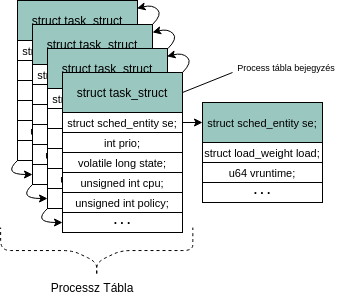
\includegraphics[scale=0.75]{images/processTable.png}
\caption{Processz Tábla}
\label{fig:structurehierarchi}
\end{figure}

\noindent A processz táblán a \texttt{for\_each\_process} makróval, egyszerűen végighaladtunk.
\begin{cpp}
struct task_struct *p;
#define for_each_process(p) \
	 for ( p = &init_task ; ( p = next_task(p)) != &init_task ; )
\end{cpp}
A \texttt{printk()}-függvényt használtam, a processz adatok naplózására.
\begin{cpp}
     for_each_process(p)
        if(!p->rt_priority)
            printk(KERN_INFO "command:%s, pid:%d, priority:%d 
            ,weight:%lu	,vruntime:%llu",p->comm,p->pid,p->prio
            ,p->se.load.weight,p->se.vruntime);

\end{cpp}

Amennyiben az ütemező módosításokat közvetlenül a kernelben szeretnénk elvégezni, a változtatások után újra kell fordítanunk a kernelt.
Ez sajnos elég hosszadalmas lehet, emiatt másik megoldást választottam.

\Section{Sysctl interfész}
A sysctl segítségével módosíthatjuk a kernel paramétereket futásidőben. Ezek a paraméterek elérhetők a /proc/sys/ jegyzékben. Emiatt a sysctl-nek szüksége van a proc fájlrendszerre. A sysctl interfész használható adatok olvasására és írására is egyaránt.

\Section{Python}
%TODO Referencia: python.org/doc/essays/blurb/
Az ütemezőn végzett módosításokból és benchmarkok programokból származó adataim feldolgozását Pythonban végzem.
A Python egy interpreteres, objektum-orientált, magas szintá programozási nyelv, dinamikus szemantikával.
A Python interpreter és a kiterjedt szabványkönyvtár, forrásként vagy bináris formátumban díjmentesen elérhető az összes főbb platformra, és szabadon terjeszthető.
A Python programok hibakeresése egyszerű: egy hiba vagy rossz bemenet soha nem okoz szegmentálási hibát.

\SubSection{Jupyter-notebook}
%TODO Referencia: https://jupyter-notebook.readthedocs.io/en/stable/notebook.html
A jupyter notebook kiterjeszti az interaktív konzol alapú megközelítését minőségileg új irányba, webalapú alkalmazás biztosításával, ami alkalmas a teljes számítási folyamat elvégzésére: kód fejlesztésére, dokumentálására és végrehajtására, valamint az eredmények közlésére.
Nagyon szimpatikusnak találtam hogy, böngészőn belüli kódszerkesztésnél, automatikus a szintaxis kiemelés, emellett pedig a behúzásokat és a böngésző füleket is szépen kezeli.
A számítás eredményének megjelenítése olyan multimédiás ábrázolókat használ mint a HTML, LaTeX, PNG, SVG stb. Például a publikációminőségű ábrák megjeleníthetők a cellákban, a matplotlib könyvtár segítségével. A LaTeX segítségével könnyen beilleszthető bármilyen matematikai képlet/jelölés a markdown cellákba.

 A notebook dokumentumai tartalmazzák az interaktív ki és bemeneteket, valamint további szövegeket, amely a kódot kísérik, de nem végrehajtásra szolgálnak. 
Emiatt a notebook fájlok, a munkamenet számítási rekordjainak egy nyilvántartása. Azaz egy fájlban megtalálható mind a futtatható kód, a magyarázó szöveg a matematikával és a kapott objektumok gazdag ábrázolásával. A dokumentum fájlokban egy JSON található és .ipynb kiterjesztéssel rendelkezik.

\SubSection{Numpy}
%TODO Referencia: https://numpy.org/doc/stable/user/whatisnumpy.html
A NumPy a tudományos számítás alapvető csomagja a Pythonban.
Ez egy Python-könyvtár, amely többdimenziós tömb objektumot, különféle származtatott objektumokat (például maszkolt tömbök és mátrixok) és rutinok széles választékát kínálja a gyors tömb műveleteihez, beleértve a matematikai, logikai, válogatást, kiválasztást, I/O , diszkrét Fourier-transzformációk, alapvető lineáris algebra, alapvető statisztikai műveletek, véletlenszerű szimuláció és még sok más.

A NumPy csomag középpontjában az ndarray objektum áll. Ez homogén adattípusok n-dimenziós tömbjeit foglalja magába, sok művelettel amit a lefordított kódban hajtanak végre a teljesítmény érdekében.
Számos fontos jellemzője van a NumPy tömböknek.
\begin{itemize}
\item A NumPy tömböket rögzített méretekkel hozhatjuk létre, ellentétben a Python listákkal.
Az ndarray méretének megváltoztatása új tömböt hoz létre, és törli az eredetit.
\item A NumPy tömb elemeinek ugyanazoknak az adattípusoknak kell lenniük, és így azonos méretűek lesznek a memóriában.
\item A NumPy tömbök elősegítik a fejlett matematikai és más típusú műveleteket nagy mennyiségű adat esetén.
\item Egyre több tudományos és matematikai Python-alapú csomag használja a NumPy tömböket, bár ezek általában támogatják a Python-szekvencia bevitelt, a feldolgozás előtt ezeket az inputokat NumPy tömbökké konvertálják, és gyakran NumPy tömböket adnak ki.
\end{itemize}

\SubSection{Matplotlib}
%TODO referencia: https://matplotlib.org/stable/index.html
A Matplotlib egy átfogó könyvtár statikus, animált és interaktív vizuális elemek létrehozásához a Pythonban.
Én a matplotlib csomagnak a pyplot részét használtam, az adathalmazaim megjelenítésére és elemzésére. A matplotlib.pyplot olyan funkciók gyűjteménye, amelyek a matplotlib-et úgy működtetik, mint a MATLAB. A függvényekkel itt, tipikusan olyan műveleteket végezhetünk mint új ábrák készítése, vonalak megjelenítése a grafikonon, az ábrázolt elem cimkékkel való ellátása, stb.

\SubSection{Pandas}
%TODO referencia: https://pandas.pydata.org/docs/getting_started/index.html#intro-to-pandas
A pandas egy gyors, hatékony, rugalmas és könnyen használható nyílt forráskódú adatelemzési és manipulációs eszköz, ami a Python programozási nyelv tetejére épült.

A NumPy indexelő operátorok [] és az attribútum operátorok gyors és könnyű hozzáférést biztosít a pandas adatstruktúráihoz. Series adatstruktúrák egyszerűen alakíthatók Numpy ndarray típusra.
Ha táblázatos adatokkal szeretnénk dolgozni, mint például táblázatokban vagy adatbázisokban tárolt adatokkal, a pandas egy megfelelő eszköz lehet. Segíthet az adatok elemzésében, tisztításában és feldolgozásában. A pandas gyakorlatilag egy keretet ad az adathalmazunknak, ezt DataFrame-nek hívják. A DataFrame egy kétdimenziós adatstruktúra, amely oszlopokban tárolhat különféle típusú adatokat (beleértve a karaktereket, egész számokat, lebegőpontos értékeket, kategorikus adatokat és egyebeket). Hasonlít egy táblázatra, SQL táblára vagy a data.frame-hez az R-ben.
A pandas segítségével grafikonon is ábrázolhatjuk az adathalmazainkat, amihez a matplotlib csomagot használja. Minden pandas által készített grafikon ábra egy matplotlib objektum.

\SubSection{Scikit-learn}
%TODO referencia: https://www.tutorialspoint.com/scikit_learn/scikit_learn_introduction.htm

A Scikit-learn (Sklearn) az egyik leghasznosabb és legerősebb könyvtár a gépi tanuláshoz, Pythonban. Széles válogatást nyújt a gépi tanulás és a statisztikai modellezés hatékony eszközeiből, beleértve a klasszifikációt, a regressziót, a klaszterezést és a dimenziócsökkentést a Python konzisztencia felületén keresztül. Ez a könyvtár, amelyet nagyrészt Pythonban lett megírva, a NumPy, a SciPy és a Matplotlib alapokra épül.
